\documentclass[12pt]{article}
\usepackage{graphicx}
\usepackage{amsmath}
\usepackage{amsfonts}
\usepackage{subfigure}
\usepackage{fullpage}
\usepackage[backend=biber, sorting=nyt]{biblatex}
\bibliography{oralrefs}
\usepackage{setspace}
\doublespace
\usepackage[font=footnotesize, labelfont=bf]{caption}
\begin{document}
\author{Michael Crumrine}
\title{CMB polarization with the Bicep and Keck experiments}
\maketitle


\section{Introduction}
The modern study of cosmology began with Einstein's publication of the general
theory of Relativity in 1915 \cite{cite:Einstein} and the development of the
Einstein field equations. In 1922 Friedmann\cite{cite:Friedmann} - assuming a homogeneous, isotropic
universe - constructed a solution to Einstein's field equation that serve as
the basis for the standard model of cosmology. In the
1930s, observations by Hubble \cite{cite:Hubble} showing the expansion of the
universe provided the first evidence of the big bang. In 1965 Penzias and
Wilson\cite{cite:Penzias} provided further evidence for a big bang origin with the discovery of
the Cosmic Microwave Background. Further observations of
the universe showed near complete flatness and uniformity on scales exceeding the
particle horizon. Then in 1981 Guth\cite{cite:Guth} suggested that a brief period of exponential
expansion now known as inflation could resolve these issues.

\subsection{History of the CMB}
The BICEP and Keck experiments observe the Cosmic Microwave Background (CMB)
which originates from photons in the early universe. In the hot big bang, the
early universe was an energetic plasma in which photons scattered continuously
from free protons and electrons which prevented propagation over large
distances. As the universe expanded, the temperature of this plasma decreased
adiabatically until the free electrons and protons could combine to form
neutral Hydrogen. After this era of recombination about 380,000 years after
the big bang, the photons decoupled from the plasma and began free streaming
through the universe in the direction of their last scattering. We observe
these photons as a 2D "surface of last scattering". 
\\
Results from COBE in 1992\cite{cite:COBE} showed the CMB to have a nearly
isotropic temperature spectrum corresponding to a 2.73K blackbody with
fluctuations on the order of 10 $\mu$K corresponding to density perturbations.
The CMB photons carry additional information besides the temperature spectrum
in the form of their polarization the first signs of which were detected by
DASI\cite{cite:DASI} in 2002. This majority of the polarization signal comes
from Thompson scattering in the inhomogeneous temperature field of the early
universe. However, an inflationary epoch would produce its own polarization
signal due to the generation of gravitational waves. The search for this
inflationary gravitational wave (IGW) signal is the ongoing target for the
Bicep and Keck program.


\section{Anisotropies in the CMB}
The near-uniform temperature spectrum of the CMB contains faint temperature
anisotropies on the order of 1 part in $10^5$. These temperature anisotropies
are largely due to - Gaussian distributed - density fluctuations at
recombination. Although we cannot predict the locations or magnitudes of these
fluctuations we can examine their statistical properties by decomposition with
the spherical harmonics:

\begin{equation}
	\delta T(\theta,\phi) = \sum _{m=-\ell} ^\ell \sum _{\ell=0} ^\infty
	a_{\ell m}Y_{\ell m}(\theta,\phi)
\end{equation}

Although this decomposition is a powerful tool, the universe is isotropic only
in a statistical sense and we therefore cannot predict any individual $a_{\ell
m}$. We instead take an average over $m$ for a given $\ell$ to form the
angular power spectrum:


\begin{equation}
	C_\ell = \frac{1}{2\ell +1}\sum _{m=-\ell} ^\ell \left< |a_{\ell m}|^2
	\right>
\end{equation}

This angular power spectrum describes the relative power of features in the
CMB according to their angular size with higher $\ell$ corresponding to
smaller features. $\lambda$

\begin{figure}
	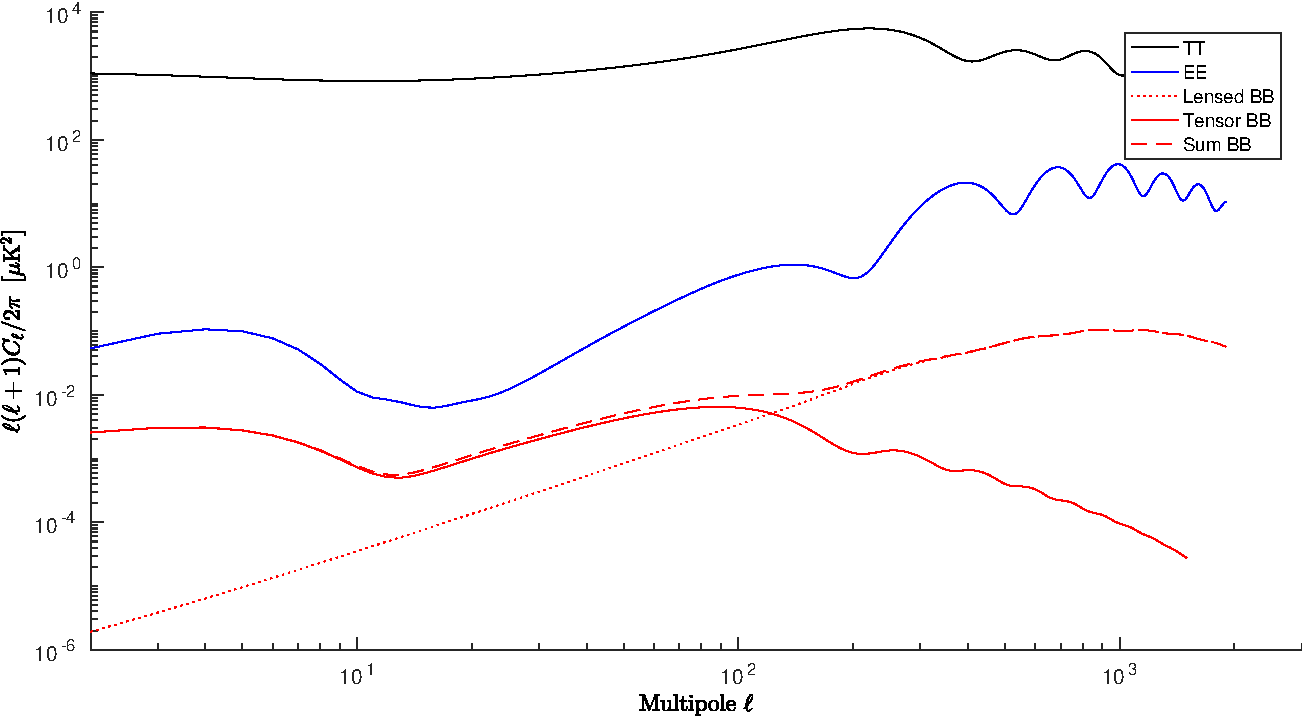
\includegraphics[width=\textwidth]{theory_aps.pdf}
	\caption{The CMB power spectrum of the $\Lambda$CDM standard model of
	cosmology as calculated by CAMB using parameters from Planck 2013. The
	temperature anisotropies (black) contain orders of magnitude more power
	than the E-mode (blue) and B-mode (red) polarization anisotropies. The BB
	spectrum is split into a lensing component (dotted) and a tensor component
	(solid) plotted at the $r=0.1$ level.}
	\label{fig:theory_aps}

\end{figure}



\subsection{Polarization Anisotropies}
\indent In addition to the temperature anisotropies that correspond to primordial
density perturbations, CMB photons are partially polarized due to Thompson
scattering in a non-uniform temperature field. This CMB polarization was predicted
at the $\approx 10\%$ level by Bond et al \cite{cite:Bond} and first detected
by DASI in 2002 \cite{cite:DASI}. Polnarev \cite{cite:Polnarev} realized that an inflationary
period would imprint an additional polarization signal on the CMB due to the
production of gravitational waves. \\
\indent This inflationary gravitational wave (IGW) signal is expected to be orders of
magnitude fainter than the signal due to Thompson scattering and difficult to
separate in the Stokes parameter space conventionally used in
Electromagnetics when studying linearly polarized light. CMB polarization
studies follow the procedures outlined in Kamionkowski et al
\cite{cite:Kamionkowski} which separates the polarization signal into a
gradient (E-mode) and curl (B-mode) component. The polarization signal
produced by Thompson scattering occurs in the presence of a temperature
quadrupole and follows the temperature gradients of the hot plasma at
recombination while the IGW signal is not restricted in this way. Thompson
scattering can therefore produce only E-modes while IGWs can produce both E
and B modes. The signal produced by these two methods is characterised by the
tensor to scalar ration $r$. Figure \ref{fig:theory_aps} shows the theoretical power spectra
of CMB perturbations in the $\Lambda$CDM standard model of Cosmology with the
addition of an $r=0.1$ IGW B-mode signal.

\section{The Bicep and Keck Program}
The Bicep/Keck experiments are a staged series of small aperture ground based
telescopes which aim to produce extremely deep degree-scale polarization maps
of the CMB. Each generation of receiver builds on the experience gained from
the previous generation while pushing deeper in sensitivity. This progression
is shown in Figure \ref{fig:BK_progression}.
\begin{figure}
	\center
	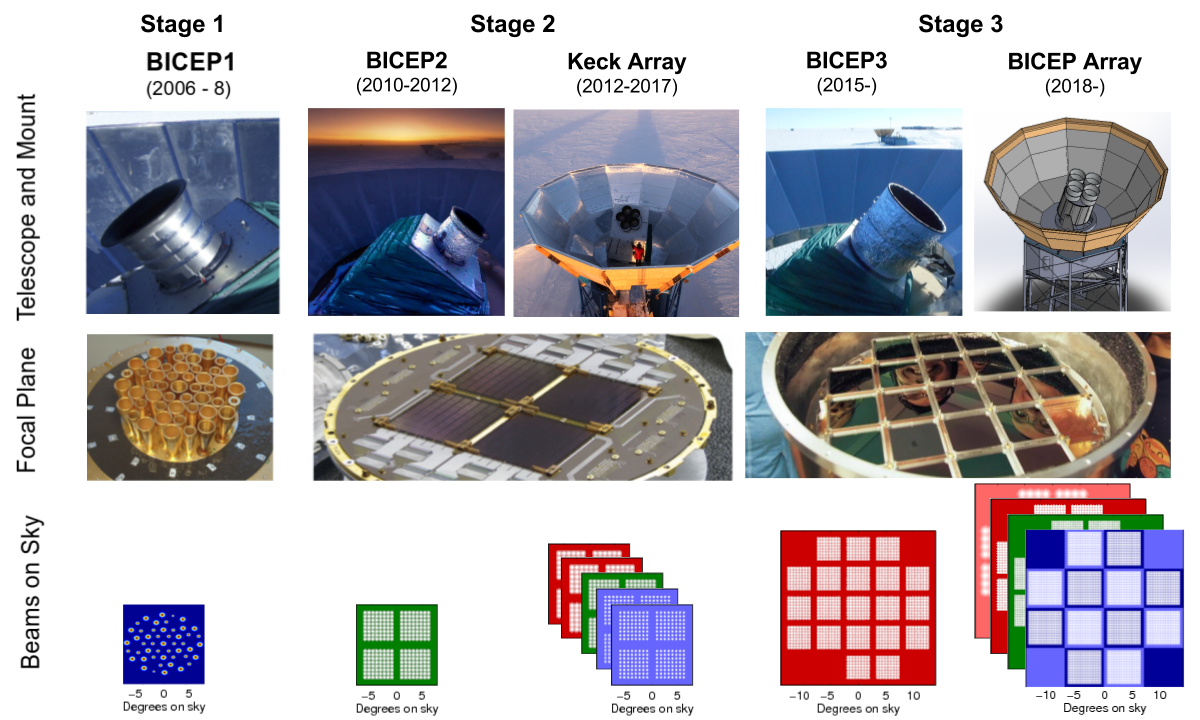
\includegraphics[width=.8\textwidth]{BK_progression.png}
	\caption{The progression of the Bicep/Keck program from Bicep1 to Bicep
	Array. The bottom row shows the beam patterns of the focal planes on the
	sky. With the exception of Bicep1 the focal plane colors correspond to
	band centers of: 35GHz - pink, 95GHz - red, 150GHz - green, 220 GHz -
	light blue, 270GHz - dark blue.}
	\label{fig:BK_progression}
\end{figure}



Bicep1 was deployed to the south pole in 2006 and used 98 feedhorn coupled
bolometers observing at 100GHz and 150GHz. Over three observing seasons the
strategies developed for observation, calibration and systematics control
proved the efficacy of small aperture refractors for CMB polarization studies
and established the leading upper bounds on inflation at $r<0.70$
\cite{cite:Bicep1}.
\\
Building on the techniques developed with its predecessor, Bicep2 replaced
Bicep1 in 2009. It exchanged feedhorn coupled bolometers for antenna-coupled
transition edge sensor (TES) bolometer arrays developed at JPL which have been
used in every subsequent telescope in the series. Concentrating its observing
power at 150GHz, in March 2014 Bicep2 announced a detection of excess signal
in its observing band consistent with an IGW signal of $r=0.2$\cite{cite:BK1}.
However, the interpretation of this excess as IGW signal relied heavily on
models of polarized dust emission which had not been highly constrained at the
time. Later that year new high frequency maps from the Planck experiment
indicated that the dust models had underestimated polarized emission in the
faintest sky regions \cite{cite:PlanckXIX}. A joint analysis with Planck and
cross correlation between the Planck 353GHz and Bicep2 150GHz maps showed that
a substantial part of the observed excess in Bicep2 was due to polarized dust
emissions \cite{cite:BKP}. This joint analysis established a new upper limit
of $r<0.12$
\\
Building on the observing power of Bicep2 the Keck Array deployed to the south
pole in 2012 with five 150GHz receivers similar to Bicep2. These additional
receivers confirmed the excess signal found with Bicep2 and contributed to the
March 2014 results. In addition to extending the Bicep2 survey depth at 150GHz
the Keck array has extended observations into three other observing bands at
95GHz, 220GHz and 270GHz. The extension into other frequencies harnesses
the Bicep/Keck program's proven capability to make deep maps to further
constrain galactic foregrounds and refine the models of polarized dust
emission. The Keck array is in its final observing season with four receivers
in the 220GHz band and one at 270GHz.
\\
In the fall of 2014 Bicep3 was deployed at the south pole to run concurrently
with the Keck array. Bicep3 vastly expands the design of the Bicep2 instrument with a
focal plane containing 2500 detectors in the 95GHz band, almost 10x the 288
detectors of a Keck style 95GHz receiver. Bicep3 serves as our prototype
instrument leading to the eventual replacement of the Keck array with Bicep
array.
\\
The Bicep array is a funded experiment which will replace the Keck Array for
multifrequency observations. Using the more powerful Bicep3 style receivers,
Bicep array will field three receivers centered at 35GHz, 95GHz, and 150GHz
along with a dual band 220/270GHz receiver. The new 35GHz receiver will
heavily constrain galactic synchrotron radiation past the upper limits set by
WMAP's 23GHZ band while the increased sensitivity at higher frequencies will
allow for better constraints on dust emissions at frequencies closer to our
other bands than the Planck 353GHz data.


\section{Multifrequency Observations}

CMB polarization experiments must be able to separate polarized foreground
signals from those imprinted on the CMB. Although these signals can be
minimized by selection of observing area their emissions must be constrained
and accounted for. As shown by the 2014 joint analysis between Bicep2/Keck and
Planck, constraints on these models have significant impact on the
interpretation of any observed excess signal. By expanding observations into
multiple frequencies, the Keck array has further constrained these dust
emissions as well as emissions due to galactic synchrotron as shown in Figure
\ref{fig:noilev}.
\begin{figure}
	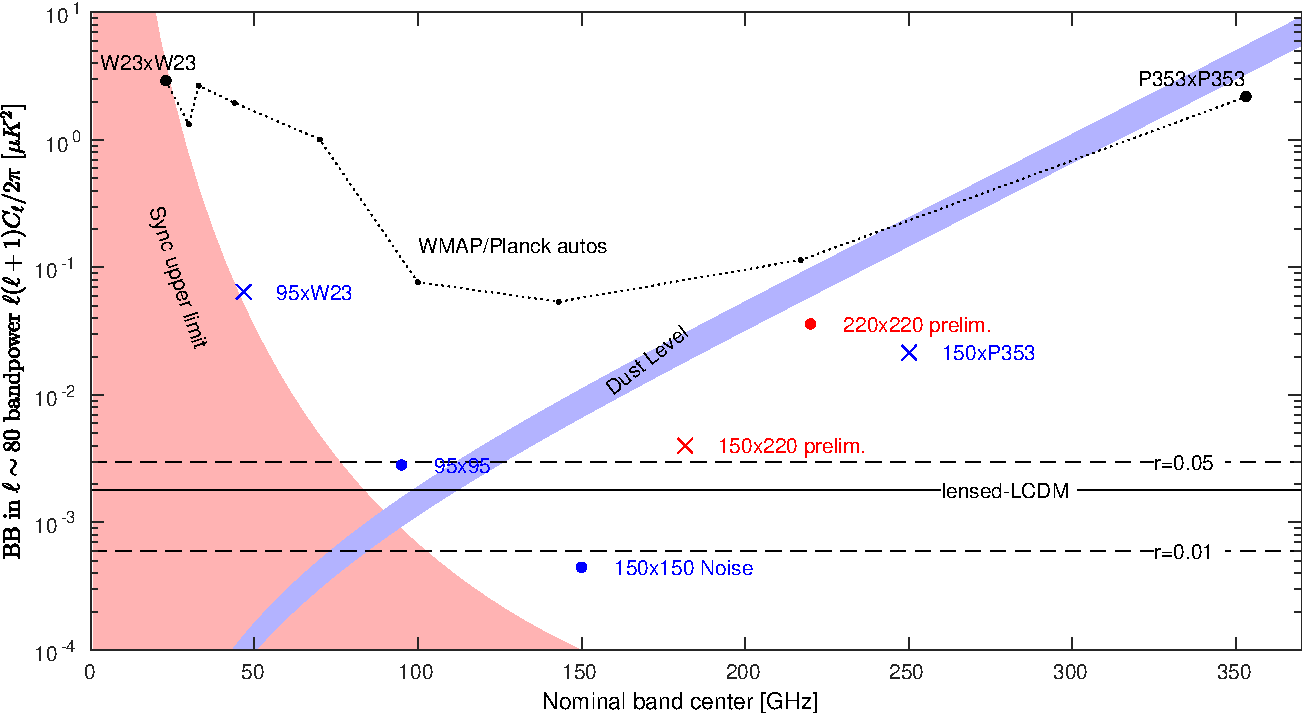
\includegraphics[width=\textwidth]{noilev.pdf}
	\caption{}
	\label{fig:noilev}
\end{figure}

\subsection{Polarized Dust}
Polarized emissions from galactic dust provide an excess BB signal on top of
that expected from $\Lambda$CDM and gravitational lensing which (although low
in power) are significant compared to the IGW signal. These emissions depend
significantly on frequency, exhibiting a power law like dependence. As shown
in Planck XXII \cite{cite:PlanckXXII} the spectral energy distribution of
galactic dust can be described by a modified blackbody spectrum

\begin{equation}
	I_d=A_d\nu ^\beta B_{\nu}(T_d)
	\label{eq:dust_sed}
\end{equation}

Where $A_d$ is an amplitude at some frequency and $\beta _d > 0$ is the spectral
index of dust emission and $B(T)$ is the standard blackbody spectrum. In order
to fully constrain the dust signal we must complement this intensity
spectrum with a description of the dust's spatial behavior

\begin{equation}
	D_\ell \propto \ell^\alpha
	\label{eq:dust_aps}
\end{equation}

where $D_\ell=C_\ell \frac{\ell(\ell +1)}{2\pi}$. The parameters in these
equations model the dust contribution to polarization signal in our field. As
Equation \ref{eq:dust_sed} shows this signal is brighter at higher
frequencies. We therefore use the Planck 353GHz maps to set these dust
parameters and extrapolate to our observed frequencies. This necessarily means
that any uncertainty contained in the high frequency observations is magnified
due to the power law behavior.

Figure \ref{fig:noilev} shows the noise uncertainty and signal levels
the $\ell=80$ bandpower where the IGW signal is expected to peak. The low 150x150
noise allows us to detect excess signal with high significance. However, the high P353xP353
noise as compared to dust signal does not provide significant enough
constraining power to separate dust signal from potential IGW signal in the
150GHz band. The 220x220 point shows preliminary numbers from our 2015
observing season in which the Keck array operated with two 220GHz receivers
and provides similar constraining power to the Planck 353GHz data while being
closer to our main observing bands. Two additional 220GHz receivers were added
for the 2016 observing season and observations at 270GHz will begin in the
current 2017 season. These observations will allow us to produce continually
improving constraints on dust in our field.
\subsection{Galactic Synchrotron}
An upper limit for an additional foreground signal is shown in Figure
\ref{fig:noilev}. Rather than increasing in intensity at higher frequencies,
polarized emissions from galactic synchrotron radiation are strongest at low
frequencies. We model synchrotron emission intensity as
\begin{equation}
	I_\nu = A_s \nu^{\beta _s}
	\label{eq:synch_sed}
\end{equation}

where $\beta _s < 0$ describes the fall off in intensity with frequency and
$A_s$ is the amplitude. The angular power spectrum of galactic synchrotron
follows the same form as dust (Equation \ref{eq:dust_aps}). The points shown
in Figure \ref{fig:noilev} mark the upper limit of synchrotron emissions as
the noise level of current observations in these bands is not sufficient for
detection. Models of the contribution due to synchrotron do not predict
significant contamination at frequencies upwards of 150GHz due to the strong
frequency dependence.
\textbf{Add in new BK15 plot with BK16 prelim points}

%Look at PIP XXX - might give more information on exactly what this beta
%parameter is. Seems like it might vary with sky patch according to BKP

\subsection{Bicep Array}

The Bicep Array experiment will leverage the technology used in Bicep3 and
expand to a multifrequency array of receivers similarly to the expansion of
the Keck array from Bicep2. 

\subsection{Detectors}
Bicep Array will continue to use the dual polarization antenna coupled
detector arrays developed for Bicep2. Each detector pixel consists of a large
number of photolithographed orthogonal slot antennas optimized for their
target wavelength. The summation of the incoming signal is eventually
deposited into a resistor, changing the temperature of the coupled Transition
Edge Sensor (TES). This produces a small change in temperature of the
on-transition superconductive element which responds with a large change in
resistance. This in turn leads to a small change in current which is amplified
through a series array of Superconducting Quantum Interference Devices
(SQUIDs) which are sensitive to extremely small changes in magnetic flux. This
use of extremely sensitive superconducting sensors allows for detection of
extremely faint CMB signal but also requires high systematics control to avoid
extraneous pickup from non-sky sources. The superconducting elements also
require a carefully designed housing in order to reach their operating
temperature of $~273mK$.


\subsection{Cryostat}

The cryogenic operating temperature of the detectors in the Bicep/Keck
experiments require carefully designed housing. Each generation of receivers
builds on the experience gained from the previous generation to improve the
design. The Bicep Array cryostats will consist of three concentric shells each
cooled to progressively lower temperatures. These shells nominally sit at
temperatures of 300K, 50K and 4K with the coolest being closest to the
center.This progressive cold shielding significantly reduces the radiative
power that is absorbed by the cooler stages which scales as $\Delta (T^4)$.
The inclusion of absorptive filters on the 300K and 50K shells help to
additionally reduce the out of band power transmitted down the optical axis.


-Widened 4K stage for extra baffling esp at 35GHZ
-Same aperture size, throughput scales with num pixels -> frequency
-Chart of pixel numbers and NETs per frequency across the receivers

\printbibliography
\end{document}
